
%!TEX root = ../master.tex
\chapter*{Intro} % (fold)
\label{cha:intro}

This document is currently under developement and none of the chapter are finish, nor in a good shape. 

This Document is a simple survey of the Machine Learning and AI method that I encounter. Most of it are based on lecture notes from my dual MSc between CentraleSupélec and Imperial College. The first goal is to be used as a personnal reminder of what I have already encounter and understood. 

The exemple below \todo{Link figure} is a scheme wich classify the machine learning algorithms in a certain way. This document does not follow this classification. 
All the definition and concept will not be explains, as a lot of ressources are available on those subjects (Computer Sciences benefits from the most open-sourced field in research). Sometimes ressources might provided, but the reader is invited to look himself for the subjects he does not understand well. 

\begin{figure}[ht]
\centering
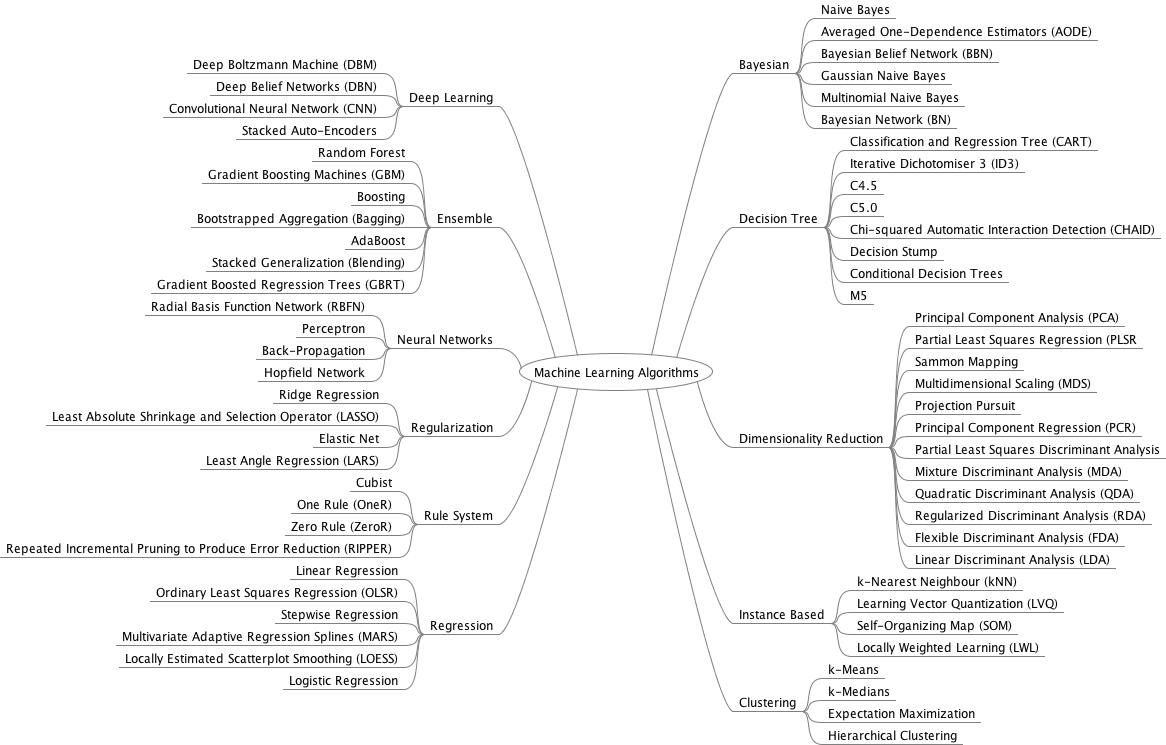
\includegraphics[scale=0.35]{figures/MachineLearningAlgorithms}

\caption{Simple graph for algorithms classification in ML}
\end{figure}

% chapter intro (end)